%
%% This is file `sample-sigconf.tex',
%% generated with the docstrip utility.
%%
%% The original source files were:
%%
%% samples.dtx  (with options: `sigconf')
%% 
%% IMPORTANT NOTICE:
%% 
%% For the copyright see the source file.
%% 
%% Any modified versions of this file must be renamed
%% with new filenames distinct from sample-sigconf.tex.
%% 
%% For distribution of the original source see the terms
%% for copying and modification in the file samples.dtx.
%% 
%% This generated file may be distributed as long as the
%% original source files, as listed above, are part of the
%% same distribution. (The sources need not necessarily be
%% in the same archive or directory.)
%%
%% Commands for TeXCount
%TC:macro \cite [option:text,text]
%TC:macro \citep [option:text,text]
%TC:macro \citet [option:text,text]
%TC:envir table 0 1
%TC:envir table* 0 1
%TC:envir tabular [ignore] word
%TC:envir displaymath 0 word
%TC:envir math 0 word
%TC:envir comment 0 0
%%
%%
%% The first command in your LaTeX source must be the \documentclass command.
\documentclass[sigconf]{acmart}
%% NOTE that a single column version may be required for 
%% submission and peer review. This can be done by changing
%% the \doucmentclass[...]{acmart} in this template to 
%% \documentclass[manuscript,screen]{acmart}
%% 
%% To ensure 100% compatibility, please check the white list of
%% approved LaTeX packages to be used with the Master Article Template at
%% https://www.acm.org/publications/taps/whitelist-of-latex-packages 
%% before creating your document. The white list page provides 
%% information on how to submit additional LaTeX packages for 
%% review and adoption.
%% Fonts used in the template cannot be substituted; margin 
%% adjustments are not allowed.
%%
%%
%% \BibTeX command to typeset BibTeX logo in the docs
\AtBeginDocument{%
  \providecommand\BibTeX{{%
    \normalfont B\kern-0.5em{\scshape i\kern-0.25em b}\kern-0.8em\TeX}}}

%% Rights management information.  This information is sent to you
%% when you complete the rights form.  These commands have SAMPLE
%% values in them; it is your responsibility as an author to replace
%% the commands and values with those provided to you when you
%% complete the rights form.
\setcopyright{acmcopyright}
\copyrightyear{2022}
\acmYear{2022}
\acmDOI{XXXXXXX.XXXXXXX}

%% These commands are for a PROCEEDINGS abstract or paper.
\acmConference[SCORES'22]{Student Computing Research Symposium}{October 6,
2022}{Ljubljana, Slovenia}
%
%  Uncomment \acmBooktitle if the title of the proceedings is different
%  from ``Proceedings of ...''!
%
%\acmBooktitle{Woodstock '18: ACM Symposium on Neural Gaze Detection,
%  June 03--05, 2018, Woodstock, NY} 
\acmPrice{15.00}
\acmISBN{978-1-4503-XXXX-X/18/06}


%%
%% Submission ID.
%% Use this when submitting an article to a sponsored event. You'll
%% receive a unique submission ID from the organizers
%% of the event, and this ID should be used as the parameter to this command.
%%\acmSubmissionID{123-A56-BU3}

%%
%% For managing citations, it is recommended to use bibliography
%% files in BibTeX format.
%%
%% You can then either use BibTeX with the ACM-Reference-Format style,
%% or BibLaTeX with the acmnumeric or acmauthoryear sytles, that include
%% support for advanced citation of software artefact from the
%% biblatex-software package, also separately available on CTAN.
%%
%% Look at the sample-*-biblatex.tex files for templates showcasing
%% the biblatex styles.
%%

%%
%% The majority of ACM publications use numbered citations and
%% references.  The command \citestyle{authoryear} switches to the
%% "author year" style.
%%
%% If you are preparing content for an event
%% sponsored by ACM SIGGRAPH, you must use the "author year" style of
%% citations and references.
%% Uncommenting
%% the next command will enable that style.
%%\citestyle{acmauthoryear}

\newcommand{\scores}{\textsc{SCORES}}

\usepackage{verbatim}
\usepackage[linesnumbered, boxed, resetcount]{algorithm2e}

%%
%% If you need any other LaTeX packages, add them here
%%

%%
%% end of the preamble, start of the body of the document source.
\begin{document}

%%
%% The "title" command has an optional parameter,
%% allowing the author to define a "short title" to be used in page headers.
\title{\LaTeX{} template for a \scores{} contribution}


%%
%% The "author" command and its associated commands are used to define
%% the authors and their affiliations.
%% Of note is the shared affiliation of the first two authors, and the
%% "authornote" and "authornotemark" commands
%% used to denote shared contribution to the research.
\author{Klemen Berkovi\v{c}}
%\authornote{All three authors contributed equally to this research.}
\email{klemen.berkovic1@um.si}
\affiliation{%
    \institution{Faculty of Electrical \\Engineering and Computer Science,\\
    University of Maribor\\Koro\v{s}ka cesta 46}
    \city{SI-2000 Maribor}
    \country{Slovenia}
}

\author{Iztok Fister Jr.}
%\authornotemark[1]
\email{iztok.fister1@um.si}
\affiliation{%
    \institution{Faculty of Electrical \\Engineering and Computer Science,\\
    University of Maribor\\Koro\v{s}ka cesta 46}
    \city{SI-2000 Maribor}
    \country{Slovenia}
}

\author{Iztok Fister}
%\authornotemark[1]
\email{iztok.fister@um.si}
\affiliation{%
    \institution{Faculty of Electrical \\Engineering and Computer Science,\\
    University of Maribor\\Koro\v{s}ka cesta 46}
    \city{SI-2000 Maribor}
    \country{Slovenia}
}

\author{Luka F\"{u}rst}
\email{luka.fuerst@fri.uni-lj.si}
\affiliation{%
    \institution{Faculty of Computer and \\Information Science,\\
    University of Ljubljana\\Ve\v{c}na pot 113}
    \city{SI-1000 Ljubljana}
    \country{Slovenia}
}

%%
%% The abstract is a short summary of the work to be presented in the
%% article.
\begin{abstract}
    This paper is a sample \LaTeX{} document that conforms to the formatting
    guidelines for the \scores\ conference proceedings.  The authors have
    tried to include a majority of commonly employed elements, such as titles
    and subtitles, footnotes, references, equations, tables, figures, lists,
    algorithms, etc.  Compile the source code of this document (the
    \texttt{.tex} file) using the \texttt{pdflatex} and \texttt{bibtex}
    commands, and compare the obtained output document (the \texttt{.pdf}
    file) with the reference document.
\end{abstract}

%%
%% Keywords. The author(s) should pick words that accurately describe
%% the work being presented. Separate the keywords with commas.
\keywords{\LaTeX, template, paper, conference \footnote{List three to ten
keywords that are specific to your paper, yet reasonably common within the
subject area of your work.}}

%%
%% This command processes the author and affiliation and title
%% information and builds the first part of the formatted document.
\maketitle

\section{Introduction}

A \emph{proceedings} is the collection of papers presented at a conference.
\scores{} seeks to produce a proceedings with a uniform, high-quality
appearance.  To this end, \scores{} imposes rigid requirements regarding the
formatting of the papers.  In particular, we prescribe a double-column format,
fonts and their sizes, margins, column width, and spacing between the two
columns.

Fortunately, \LaTeX{} automatically deals with all of these requirements.  You
only have to follow a few simple rules and make sure that the output PDF
document does not exceed \textbf{four pages}.

The remainder of this document presents a selection of \LaTeX{} commands to
specify the structure of your paper.  Rather than giving rigorous descriptions
or explanations, we present the commands through examples in the context of
this sample document.

\section{The \emph{Body} of The Paper}

Typically, the body of a paper is organized into a hierarchical structure,
with numbered or unnumbered headings for sections, subsections,
sub-subsections, and possibly even smaller sections.  The command
\texttt{\textbackslash{}section} that precedes this paragraph is part of such
a hierarchy.  By using the appropriate sectioning commands, you make \LaTeX{}
handle the numbering and placement of the headings for you.  If you want a
sub-subsection or smaller part to be unnumbered in your output, simply append
an asterisk to the command name.  Examples of both numbered and unnumbered
headings will appear throughout this sample document.\footnote{This is the
second footnote. It starts a series of three footnotes that add nothing in
terms of content but are just meant to give you an idea of how footnotes look
and work. It is a wordy footnote, so you can see how a longish one plays
out.}

Since the entire article is contained in the \textbf{document} environment,
you can indicate the start of a new paragraph with a blank line in your input
file; that is why this sentence forms a separate paragraph.

\subsection{Type Changes and \emph{Special} Characters}

We have already seen several typeface changes in this sample.  You can
indicate \emph{italicized} words or phrases in your text with the command
\texttt{\textbackslash{}emph} or \texttt{\textbackslash{}textit},
\textbf{boldface} text with the command \texttt{\textbackslash{}textbf}, and
\texttt{typewriter-style text} (e.g., for program code) with
\texttt{\textbackslash{}texttt}.  Remember, however, that you do not have to
indicate typestyle changes when such changes are part of the \emph{structural}
elements of your article; for instance, the heading of this subsection will be
in boldface, but that is handled by \LaTeX{} itself.

You can use whatever symbols, accented characters, or non-English characters
you need anywhere in your document.\footnote{The third footnote. Let's make it
rather short to see how it looks.}  You can find a complete list of what is
available in the \emph{\LaTeX{} User's Guide}~\cite{Lamport:LaTeX}.

\subsection{Math Equations}

You may want to display math equations in three distinct styles: inline,
numbered display, or non-numbered display.  Each of these styles is discussed
in the next sections.

\subsubsection{Inline (In-text) Equations}

A formula that appears in the running text is called an inline or in-text
formula.  It is produced by the \textbf{math} environment, which can be
invoked with the usual
\texttt{\textbackslash{}begin}--\text{\textbackslash{}end} construct or with
the short form \textbf{\$$\ldots$\$}.  You can use any of the symbols and
structures, from $\alpha$ to $\omega$, available in
\LaTeX~\cite{Lamport:LaTeX}.  

The inline style is not completely equivalent to the display style. For
example, as we will see in the next section, the inline equation
\begin{math}\lim_{x\rightarrow \infty}\frac{1}{x}=0\end{math} 
looks slightly different when set in the display style.

\subsubsection{Display Equations}

A numbered display equation --- one set off by a vertical space from the text
and centered horizontally --- is produced by the \textbf{equation}
environment.  An unnumbered display equation is produced by the
\textbf{displaymath} environment.

Again, in either environment, you can use any of the symbols and constructs
available in \LaTeX; this section will just give a couple of examples of
display equations.  First, consider the equation shown as an inline equation
above:
%
\begin{equation}
\lim_{x\rightarrow \infty}\frac{1}{x}=0.
\end{equation}
%
Notice that it is formatted somewhat differently in the \textbf{displaymath}
environment.  Now, let us enter an unnumbered equation
%
\begin{displaymath}
    \sum_{i=1}^{\infty} \frac{1}{x^2} = \frac{\pi^2}{6}
\end{displaymath}
%
followed by another numbered equation:
%
\begin{equation}
    \int_{0}^{\pi/2} \cos x\,dx = \sin x\bigg\rvert_{0}^{\pi/2} = \sin
    \frac{\pi}{2} - \sin 0 = 1.
\end{equation}

Next you will see an example of an unnumbered equation that is not set in the
\textbf{displaymath} environment but in short form defined with
\textbf{\$\$$\ldots$\$\$}.  When $a \ne 0$, there are two solutions to $ax^2 +
bx + c = 0$, and they are
%
$$x_{1, 2} = \frac{-b \pm \sqrt{b^2-4ac}}{2a}.$$

Here is an example of referencing an equation. Equation~\ref{equ:yannibel}
shows how to write cases in \LaTeX.
%
\begin{equation}
    \begin{aligned} 
        \mathrm{nr}(G_i,r) & = \label{equ:yannibel}
        \begin{cases}
            1  & \text{if $r$ is played by one member of $G_i$;}\\
            -2 & \text{if $r$ is not played in $G_i$;} \\
            -p & \text{if $r$ is played by $p$ members in $G_i$.}\\
        \end{cases}
    \end{aligned}
\end{equation}

\subsubsection{Long equations}

When an equation is too long for a single column, use the \textbf{aligned}
environment within the \textbf{equation} environment.  To align the equation
inside the \textbf{aligned} environment, use the symbol \textbf{\&} as seen in
Equation~\ref{equ:ho}.
%
\begin{equation}
    \begin{aligned}
        O_{\max}& = w_1 \sum_{a=1}^{m} \sum_{b=a+1}^{n} (-\lvert\text{CPT}_a 
        -\text{CPT}_b\rvert)\\ 
        &\quad + w_2 \sum_{j=1}^{m} (\text{DIF}_j) + w_3 \sum_{j=1}^{m} 
        (\text{INT}_j/\sum_{x=1}^{n} x_{ij})
    \end{aligned}
    \label{equ:ho}
\end{equation}

\subsection{Citations}

Citations to articles \cite{lecun2015deep, braams:babel, herlihy:methodology},
conference proceedings \cite{vrbancic2019transfer, clark:pct}, or books
\cite{salas:calculus, Lamport:LaTeX, fister2019computational} listed in the
Bibliography section of your article will probably occur throughout your text.
You should use \texttt{bibtex} to produce this bibliography automatically; you
simply have to insert one of several available citation commands with the key
of the item cited at the proper location in the \texttt{.tex} file
\cite{Lamport:LaTeX}.  The key is a short reference that you invent to
identify each work uniquely; in this sample document, the key is the first
author's surname and a word from the title.  This identifying key is included
with each item in the \texttt{.bib} file for your article.

The details of how to create the \texttt{.bib} file are beyond the scope of
this sample document.  More information can be found in the \emph{Author's
Guide}; for exhaustive details, see the \emph{\LaTeX{} User's
Guide}~\cite{Lamport:LaTeX}.

This article employs only the plainest form of citation, the one produced with
the \texttt{\textbackslash{}cite} command.  This is, in fact, the only
citation style recommended by the ACM.

\subsection{Tables}

Since a table cannot be split across pages, we typically place it at the top
of the page, close to its initial reference.  To achieve a proper ``floating''
placement of tables, use the environment \textbf{table} to enclose the table's
contents and caption.  The contents of the table itself have to be put inside
the \textbf{tabular} environment, which ensures a suitable alignment of rows
and columns. Again, detailed instructions on \textbf{tabular} material can be
found in the \emph{\LaTeX{} User's Guide}.

Immediately following this sentence is the point at which
Table~\ref{tab:table1} is included in the input file; compare the placement of
the table here with the table in the PDF output of this document.

\begin{table}
    \centering
    \caption{Frequency of Special Characters.}
    \label{tab:table1}
    \begin{tabular}{ccl}
        \toprule
        Non-English or Math&Frequency&Comments\\
        \midrule
        \O & 1 in 1,000& Swedish names\\
        $\pi$ & 1 in 5& In math\\ 
        \$ & 4 in 5 & In business\\ 
        $\Psi^2_1$ & 1 in 40,000& Unexplained\\
        \bottomrule
    \end{tabular}
\end{table}

To set a wider table (one that takes up the whole width of the page's live
area), use the environment \textbf{table*}.  As with a single-column table,
this wide table will ``float'' to a location deemed more desirable.
Immediately following this sentence is the point at which
Table~\ref{tab:table2} is included in the input file; again, it is instructive
to compare the placement of the table here with the table in the PDF output of
this document.

\begin{table*}
    \centering
    \caption{Some Typical Commands.}
    \label{tab:table2}
    \begin{tabular}{ccl} \hline
        \toprule
        Command&A Number&Comments\\
        \midrule
        \texttt{\textbackslash{}imagespath} & 200 & To provide the directory of included images \\
        \texttt{\textbackslash{}table} & 300 & For tables\\
        \texttt{\textbackslash{}table*} & 400& For wider tables\\
        \bottomrule
    \end{tabular}
\end{table*}

\subsection{Figures}

Like tables, figures cannot be split across pages; the best placement for them
is typically the top or the bottom of the page, close to their initial
reference\footnote{The fourth, and last, footnote.}.  To ensure a proper
``floating'' placement of figures, use the environment \textbf{figure} to
enclose the figure and its caption.

Figure~\ref{fig:circles} displays an image in the PDF format.
Figure~\ref{fig:star} shows a PNG image.

\begin{figure}
    \centering
    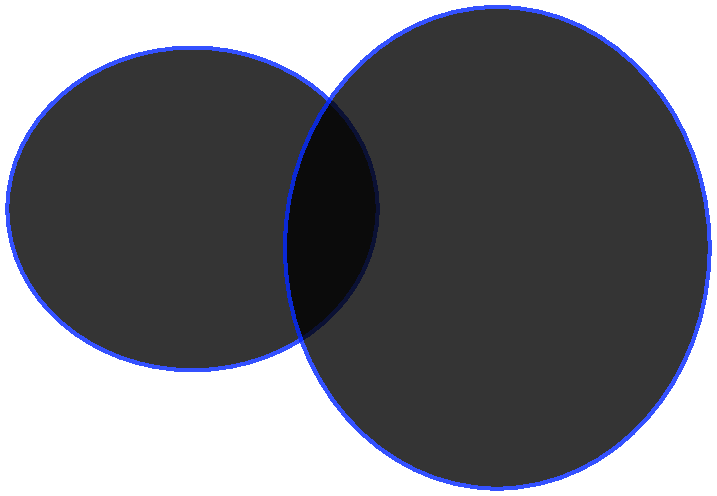
\includegraphics[scale=0.5]{circles.pdf}
    \caption{A sample circles graphic (PDF format).}
    \label{fig:circles}
\end{figure}

\begin{figure}
    \centering
    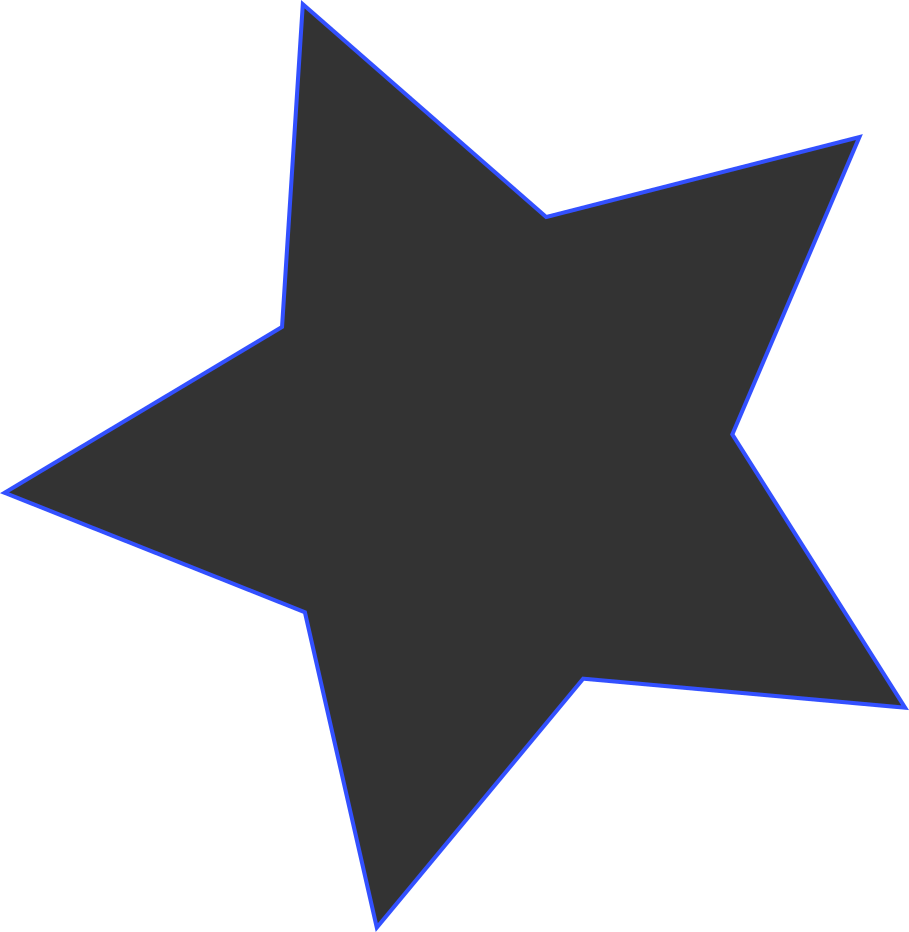
\includegraphics[scale=0.5]{star.png}
    \caption{A sample star graphic (PNG format).}
    \label{fig:star}
\end{figure}

As with tables, you may sometimes want a figure to span over two columns.  To
achieve this, while still ensuring a proper ``floating'' placement, use the
environment \textbf{figure*}.  An example can be seen in
Figure~\ref{fig:spin}.

\begin{figure*}
    \vspace{0.5cm} % we add small space, since table is being placed above the figure.
    \centering
    
\includegraphics[scale=0.8]{spin.png}
    \caption{A sample spin graphic with a span.}
    \label{fig:spin}
\end{figure*}

\subsection{Lists}

In some cases, you might want to present your ideas using lists.  Lists are
created with the \textbf{itemize} environment.  In the next example, you can
see how lists are created and used:

\begin{itemize}
    \item First item,
    \item second item, and
    \item third item.
\end{itemize}

Sometimes, authors want to reference certain list items in the subsequent
text.  For that purpose, you can use the \textbf{enumerate} environment.
Following is an example of a numbered list:

\begin{enumerate}
    \item First point,
    \item\label{list:item} second point,
    \item $\ldots$
\end{enumerate}

Item \ref{list:item} tells us what to do once we check off the preceding item.

\subsection{Algorithms}

To display algorithms in your document, employ the \textbf{algorithm}
environment.  Algorithms can be referenced in the same way as tables and
figures (e.g., Algorithm~\ref{algo:sample}).

\begin{algorithm}
    \SetAlgoLined
    \KwData{this text}
    \KwResult{how to write an algorithm with \LaTeX}
    initialization\;
    \tcc{this is a comment to tell you that we will now really start the code}
    \While{not at end of this document}{\label{algo:sample:while}
        read the current section\;
        \eIf{understand}{
            go to the next section\;
            this section becomes the current section\;
        }{
            go back to the beginning of the current section\;
        }
    }
    \caption{How to write algorithms.}
    \label{algo:sample}
\end{algorithm}

You can reference any line of your algorithm: an example of the while loop can
be seen in line~\ref{algo:sample:while}.  For more details on the \textbf{algorithm}
environment, see the
\url{http://tug.ctan.org/macros/latex/contrib/algorithm2e/doc/algorithm2e.pdf}
document.

\section{Conclusions}

This paragraph will end the body of this sample document.  Remember that you
may still give acknowledgments; a brief sample of these can be seen below.
The conclusion (or acknowledgments) should be followed by the bibliography
list (remember, the \texttt{bibtex} command produces it automatically from the
\texttt{.bib} file and the citations in your text).  To conclude, let us make
a disclaimer regarding the bibliography in this sample paper: with the
exception of the reference to the \LaTeX{} book, the citations in this paper
refer to works that have nothing to do with the present subject and are
used as examples only.

\begin{acks}
    This section is optional; it gives you room to acknowledge grants,
    funding, editing assistance, etc.
\end{acks}

\bibliographystyle{ACM-Reference-Format}
\bibliography{references}

\end{document}
